\section{Understanding Shortcut-Stacked-Encoder}\label{sec:understanding}
In this section we give analyse the sentence representations of Shortcut-Stacked Encoder\textsuperscript{$\dagger$} by visualizing how they encode (Section §\ref{sec:insights_sent_repr}) and leverage (Section §\ref{sec:insights_sent_alignment}) information from natural language text, coming from \ac{SNLI}. Additionally we show experiments, underlining the presented insights.
\subsection{Motivation}
The major downside of neural networks is the lack of interpretability \citep{goldberg2017Apr}, thus their capabilities on a lower level can only be estimated by finding meaningful evidence for their failures or sucesses on the task at hand. While analysing errors may lead to conclusions \textit{what} does not work, \textit{why} it does not work is in many cases left to intuition. Other machine-leanring classes like probabilistic or symbolic techniques do not suffer from this problem, leading to an increasing interest in visualization techniques for neural networks. Most visualitations of sentence-representations to date focus on attention-based approaches showing how words are aligned to each other such as by \cite{shen2018reinforced} or \cite{im2017distance}. To the best of our knowledge, no insights have been gained to understand the final sentence representation in vector space. In this section we demonstrate how this representation, arising from max-pooling, can be interpreted, using the Shortcut-Stacked Encoder\textsuperscript{$\dagger$} as the model to analyze. Intuitively, understanding how the Shortcut-Stacked Encoder\textsuperscript{$\dagger$} encodes information can be helpful for the task at hand of improving it using external resources. 
\newline

\noindent
While we did not manage to leverage the insights gained in this chapter to increase the performance, it might be helpful for future work.
NN nicht gut interpretierbar

\subsection{Insights on the sentence representation}\label{sec:insights_sent_repr}
In this section we show how we analyse the informaation that is present within the sentence representions, what kind of information is encoded and demonstrate, that the sentence representation can manually be adjusted in a meaningful way.
\subsubsection{Approach}
We use Shortcut-Stacked Encoder\textsuperscript{$\dagger$}, trained on \ac{SNLI}, for our analyses. This model creates for input each sentence $x$, cosnisting of words, represented as $x_i$, a sentence representation $r \in \mathbb{R}^{2048}$ with $r_j$ being the $j$th dimension of $r$. Arising from $x$, $r$ captures the relevant information for the task at hand and is used in many neural networks without a deeper understanding what each $r_j$ actually encodes. We shed light into the dimensionewise meaning of the sentence represnetation by identifying which word is responsible for the actual value of $r_j$. 
\paragraph*{Method}\label{sec:understanding1_method}
For simplicity, We explain our applied method and the reason why we use Shortcut-Stacked Encoder using a more general neural architecture of \ac{LSTM}s, a simple uni-directional \ac{RNN}.
Figure \ref{fig:rnn} (left) shows the recursive workflow of such a \ac{RNN}, following the notations of \cite{goldberg2017Apr}.
\begin{figure}[tph!]
\centering
	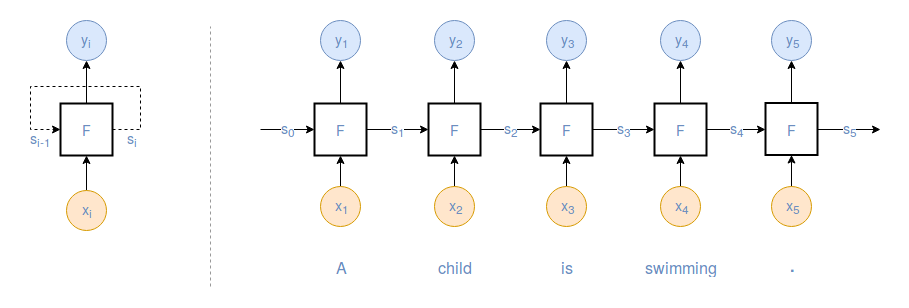
\includegraphics[totalheight=5.5cm]{fig/rnn.png}
	\caption{General architecture of a \ac{RNN} (left). Example sentence in an unrolled \ac{RNN} (right).}
	\label{fig:rnn}
\end{figure}
Maintaining an internal state $s \in \mathbb{R}^m$, for $m$-dimensional representations, the network recursively iterates over the input sequence $x$, aggregating in each timestep the previous state $s_{i-1} \in \mathbb{R}^m$ with the current input $x_i$ using the function $F$. This state is then used for the next iteration and output via a mapping function as $y_i \in \mathbb{R}^m$. Multiple implementation variants exist of $F$ and what is shared across iterations. \ac{LSTM}s for instance use several neural gates to learn what information should be used, output or forgotten. This procedure ca be seen with an example sentence yb unrolling the network in Figure \ref{fig:rnn} (right). In typial setups a neural network may either choose to use $s_t$ or $y_t$ for a sequence length of $t$ as the final sentence representation \citep{goldberg2017Apr}, since the network iterated over the full input sequence and contains the relevent information, if optimized for it. Even though the architecture of different versions of \ac{RNN} may be well understood and has a logical meaning, the actual procedure of deriving concrete representations within a trained model is hard to understand. We leverage the fact that the Shortcurt Stacked Encoder uses max-pooling over all $y_i$ to gather the sentence representation rather than using $y_t$ or $s_t$ by identifying what $y_t$ has the highest value within a given dimension and mapping this dimension to the word $x_t$ of the input sentence. As an example consider the sentence in Figure \ref{fig:rnn} (right). For each timestep $t$ a new vector $y_t$ is produced. As done by \cite{nie2017shortcut} we concatenate all $y_t$ to a matrix $\mathbb{R}^{m \times t}$, with $m$ being the representation size and each vector $y_t$ being the $t$th row within $M$. Assuming a dimensionality of $m = 3$, an examplatory matrix $M$ for the given sentence ``A child is swimming .'' is displayed in Figure \ref{fig:example_process_understanding}. 
\begin{figure}[tph!]
\centering
	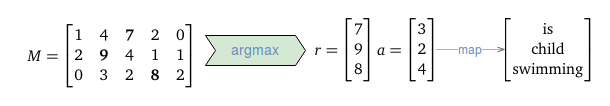
\includegraphics[totalheight=2cm]{fig/example_process_understanding.png}
	\caption{Visualized example of extracting interpretable information of the max-pooled seentence representations with a dimensionality of 3.}
	\label{fig:example_process_understanding}
\end{figure}
Additiobnally to creating the sentence representation $r$ by applying wor-wise max-pooling on $M$, we collect the vector $a$, containing the column indizes, that are responsible for the values within $r$. These can directly be mapped to the word of the source sentence and thus be interpreted by humans. It should be notted that due to the nature of the multi layer \ac{biLSTM} each $y_t$ does not only contain the word at $x_t$ but its context. While this somehow may lead to less accurate mapping, we found that the chosen method is sufficient to gain some meaningful insights on sentence encoding.

\paragraph*{Analysed data}\label{sec:understanding1_analysed_data}
To reduce noise and aming for sentences that Shortcut-Stacked Encoder\textsuperscript{$\dagger$} seems to have a proper understanging about, we sample 1000 sentence representations from the \ac{SNLI} train data in the following strategy. We group all sentence pairs ($p$, $h$) sharing the same premise and only keep groups if all samples belonging to the same group are classified correctly. Thus, we reduce the amount of sentences that are definetly misunderstood by the model, that would be harder to interpret. For now we are not interested in the actual relation between $p$ and $h$ and therefore create a pool of the remaining sentences, by treating $p$ and $h$ equally and splitting their connections apart. After removing duplicate sentences, the most frequent sentence length for the remaining representations is 8. To reduce noise that may arise from different sentence lengths, we only consider sentences of a length of 8 and randomly sample 1000 sentence representations. All experiments in this chapter are based on the same instances, unless otherwise stated.
\newline

\noindent
In addition to the representation values each sample contains the following information:
\begin{itemize}
\item \textbf{Token:} The tokens that triggered the maximum value for the representation.
\item \textbf{Token position:} Positional information about the responsible tokens within the sentence.
\item \textbf{Lemma:} The lemmata of the responsible tokens.
\item \textbf{\ac{POS}:} The \ac{POS} tags of the responsible tokens.
\item \textbf{Dependency Parse:} The tags of the responsible tokens within the dependency parse tree.
\end{itemize}
Lemmatizing, \ac{POS}-Tagging and dependency parsing were conducted using spaCy\footnote{\href{https://spacy.io/}{https://spacy.io/}}.

\subsubsection{Detection of relevant dimensions}
As commonly done when analysing data we start by showing a rough look into the sentence representations at hand. Typically, the \ac{SD} within a dimension correlates with the with the relevance for decision making. Naturally, a dimension that does not change its value and thus being close to a constant is not informative, while a value with a high \ac{SD} can be considered informative \citep{Bishop2007}. We calculate \ac{SD} over all dimensions, depicted as a histogram in Figure \ref{fig:sd}.
\begin{figure}[tph!]
\centering
	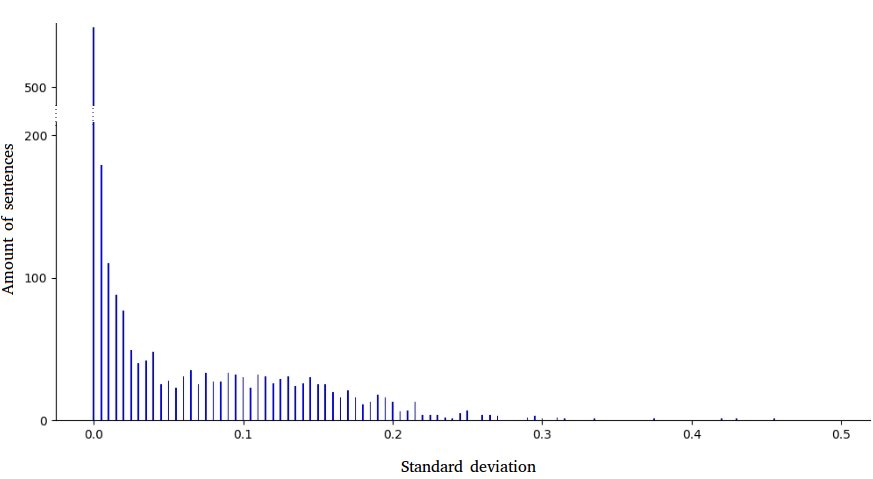
\includegraphics[totalheight=8cm]{fig/sd.png}
	\caption{The standard deviation within a dimension of sentence representations (x-axis) by the amount of dimensions with the given standard deviation.}
	\label{fig:sd}
\end{figure}
We plot the standard deviations in a discrete space using a bin size 0.05. For each if the 2048 dimensions we calculate its \ac{SD} to assign them to the correct bin. The amount of dimensions with the given \ac{SD} is shown on the y-axis, note that the upper part of the plot is truncated for the sake of compactness. As can be seen, only a very tiny fraction of the dimension shows a large variation, the vast majority contains more or less the same value, regardless of the sentence. This obviously  does not mean, they contain no information at all, as they may only be used to encode information that is rarly present within the data, however itserves as a reliable source, what dimensions are relevant to the model.

\paragraph*{A naive approach to identify dimensional encoding}
An intuitive approach to identify, what is encoded within the sentence representation, is to find common similarities between the words across all sentences, that are responsible for the according dimmension. Especially the task of \ac{NLI} we assume \textit{semantic}, \textit{syntactic} or \textit{positional} information to be required. Those can all be inferred using the features we extraced in Section §\ref{sec:understanding1_analysed_data}. Similarities between words heavily depend on the context they appear in \citep{dagan2000contextual}. For instance one could consider a car and an identical recunstruction in original size of the same car as similar, whereas a horse is very distinct. Adding additional information that one needs to reach a destination in short time, he or she is more likely to consider the horse similar to the car, desicing between these two option. This essentially comes to a major problem when investigating semantic encoding without prior knowledge of what attributes may be considered relevant. We therefore investigate the sentence representation using excessive manual search in a top down manner, by first searching for patterns across all dimensions. In Section §\ref{sec:understanding2} we will look into some dimensions in detail.

\paragraph*{A tool for sentence representation visualization}
In order to evaluate many patterns with minimal time effort, we create a visualitazion tool, capable of dynamically generating any labelling scheme for responsible words based on the features descried previously. A sample visualitation is shown in Figure \ref{fig:find_position_1}.
\begin{figure}[tph!]
\centering
	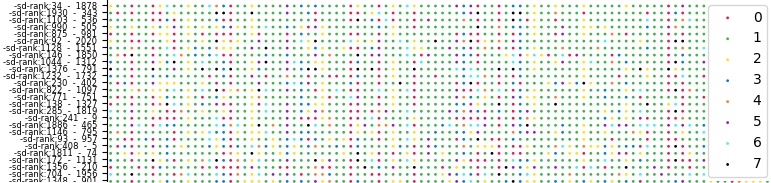
\includegraphics[totalheight=4cm]{fig/finpone.png}
	\caption{An extraction of a grid-plot, showing dimensions with the position within the sentence of the word, responsible for the dimensional value.}
	\label{fig:find_position_1}
\end{figure}
This grid-plot visualizes for each row the responsible words for one dimension, listed on the right side as (\texttt{<rank in terms of \ac{SD}}\footnote{All dimensions are ranked by their \ac{SD}, giving an intuition of the expressiveness of the dimension.}\texttt{> - <dimension index>}), colored based on the attributes of interest. In this particular case words are colored by their position within the sentence.  Each column refers to the same sentence along different dimensions. As a trade-off between explanatory power and clarity we always plot 300 sentences on 300 dimensions, which are eigther oredered by \ac{SD} or already pre-sorted by the frequency\footnote{Even though we only use 300 sentences and dimensions for plotting, calculatiions are based on all the selected data.} of a label of interest. In this particular case, dimensions are ordered by their frequency of words on the üposition 1, meaning the upmost dimension received its values from the second word (index $1$) more than any other dimension. Looking for patterns across many sentences, we focus on horizontal lines with the same coloring or colors referring to attributes that may be interpreted similarily. Vertical lines indicate different differences across sentences with respect to the attribute of interest.


\paragraph*{Interpretation of positional Information}
Word-ordering is crucial  with respect to the meaning of a sentence. We evaluate if ceertain dimensions are aligned to specific word positions, only meant to encode the meaning of the word at this place. Figure \ref{fig:find_position_1} shows dimensions that are heavily influenced by the second word, indicated by the vast majority of green dots. And indeed, several also very informative dimensions are dominated by the second word of a sentence with some noise, primarily stemming from other word positions from the beginning of the sentence. Considering the nature of sentences of \ac{SNLI}, as presented in Section §\ref{sec:snli}, this is however not enough evidence to conclude, those dimensions correspond (solely) to positional information within the sentence. Consisting merely of simple sentence structures of even only phrases it is very likely that the second word corresponds to a noun, most likely describing the main aspect of the image. Optional preceding articles or adjectives may cause this noun to have varying positions between one and three. Looking at the coloring of vertical lines this assumption is backed, as for each sentence, the responsible word arises fairly consitstently from the same position across dimensions, indicating that this stems from the encoded attribute rrather than noise. In general we find no meaningful\footnote{We do find several dimensions that mostly arise from the first word, yet the resulting value is mostly constant across all sentences and stems mainly from articles.} dimensions ecoding solely positional information, either absolute or relative, without being correlated strongly with another attribute.
\paragraph*{Finding syntactic dimensions}
This warrants more investigation using a different labeling scheme, and we look for clues based on the \ac{POS} tags. Tokens are labelled using the Penn Treebank Part-of-Speech Tagset \citep{marcus1993building} and present in our data with the originally assigned labels. Figure \ref{fig:find_syntax} shows an extract of dimensions labelled by \ac{POS} tags, pre-sorted such that dimensions with any single dominant label are shown first. We aggregate different \ac{POS}-tags refering to the same concept together, thus for instance all nouns \texttt{NN}, \texttt{NNS}, \texttt{NNP} and \texttt{NNPS} are all labelled as \texttt{NN}. Several patterns can be seen within this plot especially punctuation seems verly well presented at first sight (green and orange). Looking into the actual data and considering their very low \ac{SD}, these dimensions seem in fact less important. We observe similar issues for dimensions that are dominated by articles (orange). More interestingly are nouns (yellow), being very dominant in diverse dimensions, including dimension \textit{1878} (fourth row), which also was well represented by the second word when checking for positional information (first row in Figure \ref{fig:find_position_1}). 
\begin{figure}[tph!]
\centering
	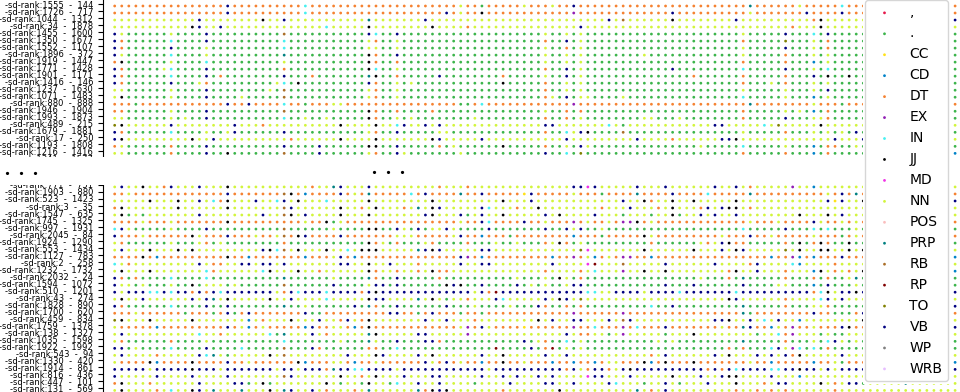
\includegraphics[totalheight=7cm]{fig/finsynpos3.png}
	\caption{An extraction of a grid-plot, showing syntatical information using the \ac{POS} tag with pre-sorted rows to have a single dominant label.}
	\label{fig:find_syntax}
\end{figure}
\noindent
This supports our intuition that word positions are not directly encoded but merely correlated to other features, like an early noun in this case. Also verbs (blue) are well presented in two dimensions. This plot suggests that indeed that model caütures syntactic information to some extend, represented within the according dimensions respectively, however also shows some drawbacks of our initial naive approach:
\begin{enumerate}
\item \textbf{Correlation:} As we have shown different attributes may correlate with each other, thus it is unclear if a found pattern is merely a side product of a correlated feature or the main thing being encoded by a dimension.  
\item \textbf{Non existent information:} Interpreting the meaning of a dimension by the responsible word is only possible if this word indeed characterizes the dimension. In case of positional information we can be certain, that each sentence contains a word that reflects the information with respect to our labeling scheme, as every sentence contains words with all positions. However when looking for encoded information that is not present amongs all sentences, another arbitrary word will still be responsible for the dimension's value. In our caase when finding syntactical clue for instance, most sentences have punctuation, nouns, determiners or verbs. A dimension representing adjectives however will alsways look very noisy, as it can only be represented by adjectives in sentences containing one.
\item \textbf{Representation value:} We did not yet consider the actual representation as used by the model for prediction. Especially considering the previous issue, we expect the model to have some kind of encoding to differentiate, whether the information of a dimension is present or not.
\end{enumerate} 
While we will never completely get rid of the first issue, we try to remedy misinterpretations coming from all three issues by closely analysing dimensions separatley in Section §\ref{sec:understanding2} together with the actual values of $r$ in the dimension at hand. We reduce the shortcomings from the second issue by adding a filtering option, that we demonstarte in the next section by identifying dimensions containing semantic information.

\paragraph*{Finding semtantic dimensions}
Looking at the actual data we observe that several dimensions only include words referring to female humans. We investigate this finding by looking for dimensions that contain gender-specific information. Based on the data we create two wordlists for female\footnote{Words in the \textbf{female} wordlist: \textit{daughter, daughters, female, females, girl, girls, lady, mother, mothers, her, herself, she, sister, sisters, wife, woman, women}} and male\footnote{Words in the \textbf{male} wordlist: \textit{boy, boys, dude, father, grandfather, guy, guys, he, him, himself, his, husband, male, males, man, men, son, sons}} humans respectively. Following our observation, that more specific information causes more noise in the visualitation due to sentences not containing it, we only consider sentences containing at least one word from at least one wordlist. The resulting plot is depicted in Figure \ref{fig:find_male_female} with dimensions sorted by their informativeness according to \ac{SD}. Words are labelled as \textit{male} or \textit{female}, if they occur in the according wordlist, any other word than those is labelled \textit{OTHER}.
\begin{figure}[tph!]
\centering
	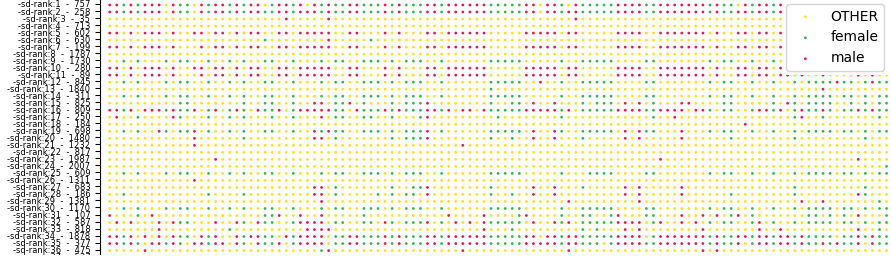
\includegraphics[totalheight=5cm]{fig/findmf.png}
	\caption{An extraction of a grid-plot, gender specific female using only sentences with words of pre-defined wordlists.}
	\label{fig:find_male_female}
\end{figure}
Several interesting findings are shown here. The first two dimensions having the highes variation do not distinguish between female or male humans, but instead jointly encode both information, seemingly focusing on humans having a gender. We will look closer into these dimensions in Section §\ref{sec:understanding2}. More importantly however, we observe several dimensions with only male (red) and OTHER (yellow) words responsible for its value, while others only arise from female (green) and OTHER only. Comparing these dimensions we see, that some of them are strongly complementary to each other with respect to the encoded gender: We interpret dimensions that exclusively retrieve their values from female or OTHER words to encode whether there is a female human being present in the sentence (labelled as female) or not (labelled as OTHER). Similarily, dimensions exlusively arising from male or OTHER words are likely to encode whethere a male human being is within the sentence or not. Based on this interpretation one can observe that male-encoding dimensions are labelled as OTHER exactly in those dimensions, that are labelled as female in female-encoding dimensions and vice versa. Note that all displayed dimensions contain the highest overall \ac{SD}, indicating that they are amongst the most expressive dimensions of the model. Being redundantly in several informative dimensions encoded, we conclude, that gender-specific information is highly relevant for \ac{SNLI}. This observation is in line with \cite{gururangan2018annotation}, who show that removing the gender information to create the hypothesis was a common heuristic applied by the annotators when creating the dataset.

\subsubsection{Female and male dimensions}\label{sec:understanding2}
We rely on the method described above to manually find patterns that are encoded in the sentence representations and identify the vorresponding dimensions. Following the drawbacks of our naive approach we conduct our dimension-wise analysis with respect to the actual values of the given dimension, that are retrieved from each word. We represent each dimension in a histogram by mapping the dimensional values from each sentence into a descrete space. In prelimitary attempts tried to automatically divide the one-dimensional feature space of a dimension into meaningful intervals, however this did not create meaningful representations. 
\paragraph*{Female and male dimensions}
Subsequently to the findings in the previous section, Figure \ref{fig:mf_basic} shows a detailed view of one of the male-encoding dimensions with no filter applied, thus using all 1000 sentences. For each sentence we retrieve the value of the two displayed dimension and assign it into bins of size $0.05$ displayed on the x-axis. The amount of sentences containing a specific value is displayed on the y-axis for each bin, colored by the chosen labelling scheme. Based on our previous observation we assume the gender-dimension to only encode whether  a human with the given gender is within the sentence or not. To ensure, terms for humans without a gender are not presented in those dimensions we create  third category, containing words for humans regardless of their gender \footnote{Words in the \textbf{gender-less} wordlist: \textit{parent, parents, friend, friends, person, people, familiy, student, adult, adults, couple, couples, child, children}}. Additionlly we move pronouns from our previous wordlists into new categories. 
\begin{figure}[tph!]
\centering
	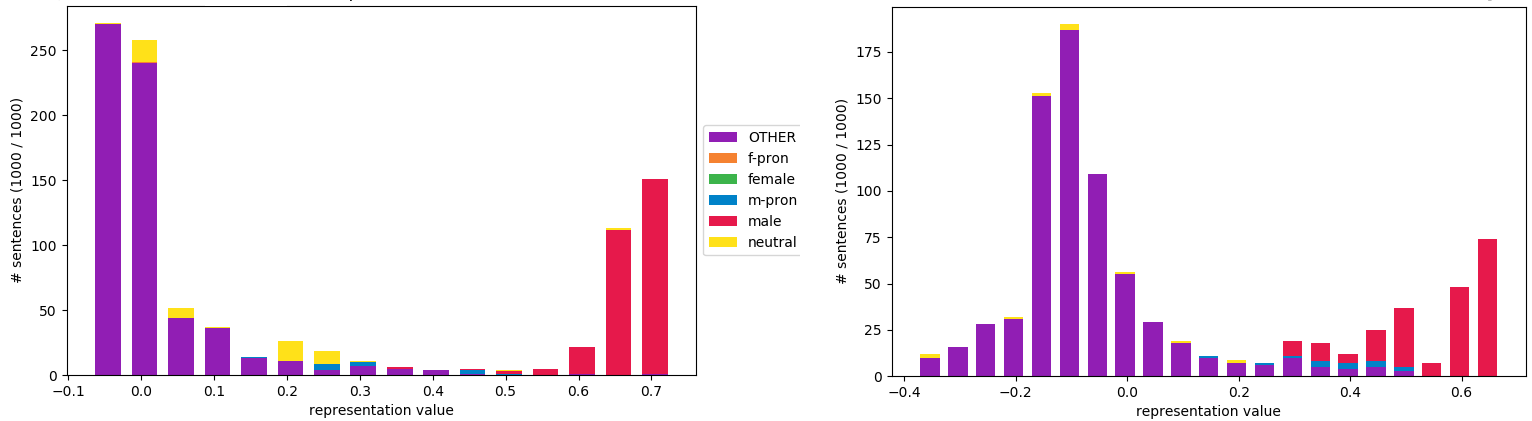
\includegraphics[totalheight=4.5cm]{fig/mf_basic.png}
	\caption{Representation visualitation with respect to genders of dimension 199 (left) and dimension 602 (right).}
	\label{fig:mf_basic}
\end{figure}
Both dimensions undermine our initial assumption that they encode whether a male human is present within the sentence or not. Clearly this is seperated by the value within the dimension. While all high values arise from male words, most of them covered by our rather limited wordlists, not a single value stems from any word of the female wordslists. While neutral words may be responsible for values within these dimensions, their influence is negligable. All words coming from lower-valued bins seem arbitrary, arising from the fact that some sentences do not contain any male words and thus a random word will take its place, resulting in a low value. Even though the distributions are different, both presented dimensions seem to encode the same information. For an even more detailed view, we focus on the individual words from our male wordlist in Figure \ref{fig:mf_detailed_m}.
\begin{figure}[tph!]
\centering
	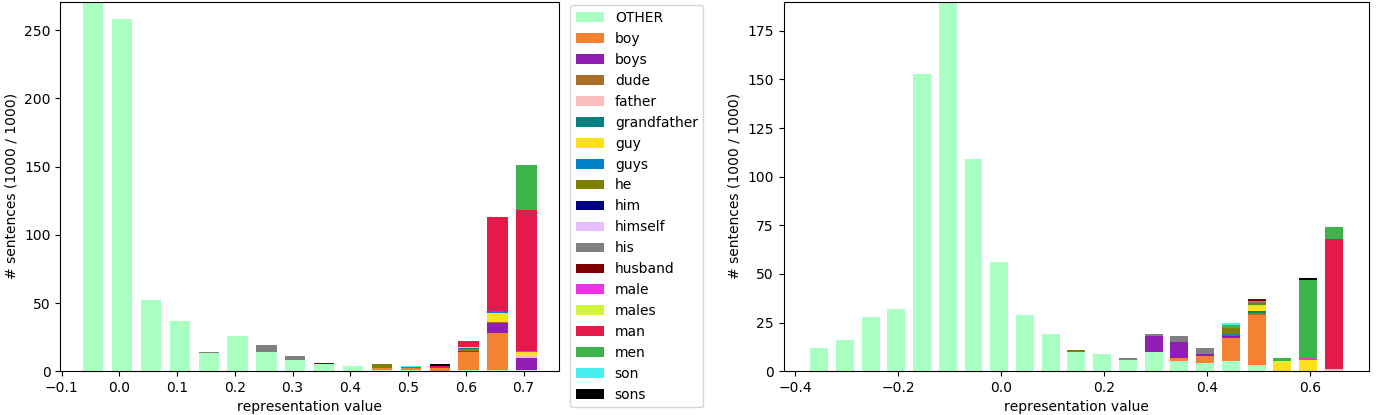
\includegraphics[totalheight=4.5cm]{fig/mf_detailed.png}
	\caption{Detailed representation visualitation of different terms for human males of dimension 199 (left) and dimension 602 (right).}
	\label{fig:mf_detailed_m}
\end{figure}
We observe, that both dimensions enable a fine-grained differentiation between different words and their meanings, even within their high values. In both cases, \textit{boy} scores a lower value than \textit{man} as being ``less male'', indicating that this dimension not corresponds to the biological male gender but to attributes are generally assoziated with males. This only seems logical, as it is known that gender information is present in distributed word-representations \citep{mikolov2013linguistic} that our model relies on. These again are determined by their surrounding context, which obviously is dominated by male-\textit{assoziated} words. While both dimension seem to encode the same information, based on the words reaching high values, the encoding of this information slightly differs. Dimension 199 has the tendency to score higher values if multiple males, namely \textit{boys} and \textit{men}, are present, whereas dimension 602 reduces the value for plurals. 
\newline

\noindent
We simillarily investigate the female-endocding dimensions, depicted in Figure \ref{fig:mf_detailed_f} already using the detailed labelling and observe the same principal encoding scheme. 
\begin{figure}[tph!]
\centering
	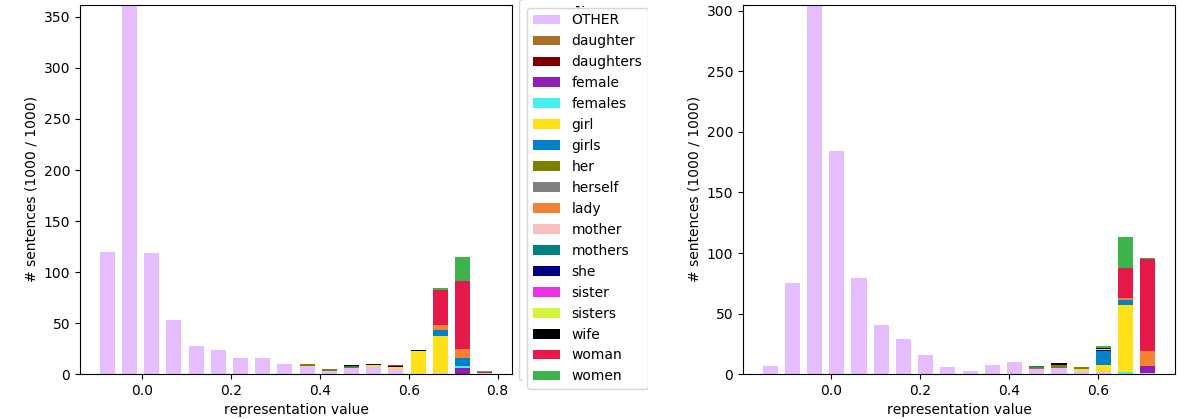
\includegraphics[totalheight=5cm]{fig/mf_detailed_f.png}
	\caption{Detailed representation visualitation of different terms for human females of dimension 845 (left) and dimension 311 (right).}
	\label{fig:mf_detailed_f}
\end{figure}
As for the male-encoding dimensions, all higher values within both dimensions arise almost exclusively from our female wordlists. Younger females, namely \textit{girl[s]}, are encoded using a lower value than \textit{woman} or \textit{women}. Furthermore, the different encoding of both female dimensions of singular and plural is aligned with the differences depicted in the male dimensions. Subsequent visualitations of other dimensions show similar results, such that highr valued words may easily grouped by some attributes while low values words seem rather arbitrary. We conclude that a dimension, encoding any kind of specific information $i$, by ssigning high values, if $i$ is present within the sentence and low values if $i$ is not given. Note that this explanation intuitively can be aligned with the max-pooling. Given that $i$ is within the sentence, the model adjusts its weights such that the dimensions encoding $i$ will result in high values, which naturally will be selected as being the highest amongst all values. In case $i$ is not within the sentence any other arbitrary word will have the highest value of the specific dimensions, however this will be significantly lower than in the previous case. We show further evidence for this explanation in some remainding subsections.

\paragraph*{Relevance of female and male dimensions}
\begin{wraptable}[12]{r}{7cm}
%\begin{table}[]
\centering
\label{tab:relevance_mf_nn}
\begin{tabular}{llll}
\textbf{$|r|$} & \begin{tabular}[c]{@{}l@{}}\textbf{MLP}\\ \textbf{size}\end{tabular} & \textbf{Acc. (train)} & \textbf{Acc. (dev)} \\
\toprule
2 & 6& 42.26\% & 42.87\%\\
4 & 12& 47.11\%& 47.41\%\\
6 & 18& 47.50\%& 48.64\%\\
8 & 24& 49.54\%& 50.37\%\\
\bottomrule      
\end{tabular}
\caption{Accuracies achieved on \ac{SNLI} using $|r|$-dimensional sentence representations of gender-specific dimensions.}
%\end{table}
\end{wraptable}
We want to gain information of how relevant those identified dimensions actually are when the predicting the relations on \ac{SNLI}. Thus we conduct an experiment with sentence representations solely consisitng of dimensions that we identified to encode gender-specific information. Specifically we found four dimensions to encode each gender respectively. We only consider subsets of these dimensions as sentence representations and train for each subset, consisting of an equal amound of female and male dimensions, a new model for 5 iterations using the same hypeerparamters as in the Shortcut-Stacked Encoder\textsuperscript{$\dagger$}. Solely the size of the hidden layer is changed with respect to the size of the sentence representation due to being trmendously reduced. The results in Table \ref{tab:relevance_mf_nn} show that a sentence representation solely consisting of one dimensio per gender reaches an improvement of about 9 points in accuracy over a random baseline with 33.33\%. Adding more dimensions somehow reduced the additional improvements, indicating some redundancy but also some distinct information encoded within those dimensions. About half of the data can be classified correctly based on only 8 dimensions encoding gender-information of the sentence. This may indicate that these dimensions are highly relevant within the model, however all these observations may also arise from the model learning patterns, that are not considered by the original model. We thus conduct another experiment to shed more light into the impact of the detected dimensions.

\paragraph*{Inverting gender information in the sentence representation}
Knowing what information is encoded and how this is done we try to twist the sentence representations before theey are fed into the classifying \ac{MLP}, to see if it is possible to exploit the gained knowledge for adjusting the represented meaning withou adapting the actual input sentences. Specifically we try to inveert the meaning of the found gender-specific dimensions: If the sentence representation originally contains information that a male or female human is present, we change it to be not present and vice versa. Let $d^i_j$ denote the value of the $i$th dimension within the $j$th sentence representation. For all $i$ referring to gender-encoding dimensions\footnote{\textbf{Male} dimension indizes: 89, 199, 280, 602; \textbf{Female} dimension indizes: 311, 609, 845, 1730} we calculate the maximum reached value $d^i_{max}$ and minimum reached value $d^i_{min}$ over all $n$ sentences:
\begin{equation}
d^i_{max} = \arg\max_{v^i}(v^i | v^i \in \{d^i_0, d^i_1, \cdots,d^i_{n-1}, d^i_n\})
\end{equation}
\begin{equation}
d^i_{min} = \arg\min_{v^i}(v^i | v^i \in \{d^i_0, d^i_1, \cdots,d^i_{n-1}, d^i_n\})
\end{equation}
We further calculate the new value $\bar{d}^i_j$, replcing the original value $d^i_j$ for all relevant $i$ using the following equation. Note that we replace $d^i_j$ by $\bar{d}^i_j$ prior to the feature concatenation, ensuring to overwrite all relevant features. Basically we mirror each value on the dimension's mean, ensuring that the resulting values are within the common range for the given dimension.
\begin{equation}\label{eq:invert}
\bar{d}^i_j = \frac{d^i_{max} + d^i_{min}}{2} + \left(\frac{d^i_{max} + d^i_{min}}{2} - d^i_j\right) = d^i_{max} + d^i_{min} - d^i_j
\end{equation}
Rather than using the sample mean from all sentences, which would be heavily influenced by how much the encoded information is represented within the data, we calculate the mean based on the outer values, intending to focus on the information-encoding aspect. Considering the distributions of the dimensions having two peaks, either low or high valued, we assume this method to be appropriate for our experiment.

\paragraph*{Evaluation of inverted gender-dimensions}
We use the evaluated the proposed method in the full \ac{SNLI} train and dev data and report our results in Table \ref{tab:inverted_mf_results_acc} together with the original performance of the used Shortcut-Stacked Encoder\textsuperscript{$\dagger$}. 
\begin{table}[tph!]
\centering
\label{tab:inverted_mf_results_acc}
\begin{tabular}{cccccc}
\textbf{Inverted dimensions} & \textbf{Inverted sentences}  & \textbf{Acc. (train)} & \textbf{Acc. (train) +/-} & \textbf{Acc. (dev)} & \textbf{Acc (dev) +/-} \\
\toprule
None                   & None                   & 87.41        & 0.0              & 85.31      & 0.0           \\
\midrule
1 female, 1 male    & premise, hypothesis & 87.36        & -0.05            & 85.25      & -0.06         \\
2 female, 2 male    & premise, hypothesis & 87.25        & -0.16            & 85.19      & -0.12         \\
3 female, 3 male    & premise, hypothesis & 87.08        & -0.33            & 84.97      & -0.34         \\
4 female, 4 male    & premise, hypothesis & 86.82        & \textbf{-0.59}            & 84.78      & \textbf{-0.53}         \\
\midrule
1 female, 1 male    & hypothesis          & 87.05        & -0.36            & 84.73      & -0.58         \\
2 female, 2 male    & hypothesis          & 84.76        & -2.65            & 82.29      & -3.02         \\
3 female, 3 male    & hypothesis          & 80.23        & -7.18            & 78.28      & -7.03         \\
4 female, 4 male    & hypothesis           & 73.20        & \textbf{-14.21}           & 71.69      & \textbf{-13.62}    \\
\bottomrule    
\end{tabular}
\caption{Results in terms of accuracy of inverted gender-specific dimensions on \ac{SNLI} train and dev set.}
\end{table}
The table shows a range of experiments with an increasing number of dimensions being inverted on either both sentences or only the hypothesis. It can be seen that even after inverting all four dimensions for each gender, the performance only slightly drops, when applied on both sentenes. this indicates that the performed equation (\ref{eq:invert}) indeed is sufficient to invert the encoded information to a high degree, since inverting the gender in $p$ and $h$ simultaneously should not have an impact on the final prediction\footnote{We select only 8 out of 2048 dimensions, that are highly representative for the gender-specific meaning. Correlated information however also has an impact on other dimensions that we left untouched, thus we don't claim to have inverted the full gender-specific meanung, but a crucial amount of it.}. More importantly, when only the hypothesis' representation is changed, we observe that inverting a single dimension reduces the model's performance only slightly. An increasing amount of inverted dimensions also increases the impact on the overall accuracy. We conclude that  this is due to redundant information, most likely coming from dropout. 
\paragraph*{Analysis of inverted gender-dimensions}
In order to actually see that sentence meanings shifted according to our expectations, namely male individuals should be intereted as female and vice versa, we analyse the actual predictions of the data. the results for our observations when looking for differences between the models prediction using the untouched or inverted (using all eight dimensions, inverting the hypothesis only) sentence representations are shown in Table \ref{tab:inverted_mf_results_samples}.The upper part of the table depicts samples with human main actors having gender that re correctly classified by the original model. By inverting the mentioned dimensions we invert the gender-aspect of these actors abd subsequently a \textit{woman} in the hypothesis is actually interpreted similarily to a \textit{man} by the model. We observe that the vast majority of samples containing the same gender in premise and hypothesis flip the predicted label after following this interpretation. Some samples without explicit gender information, like \textit{dog} in thwe lower part of the table, remain with the same label. 
\begin{table}[tph!]
\resizebox{\textwidth}{!}{%
\centering
\label{tab:inverted_mf_results_samples}
\begin{tabular}{llcc}
\textbf{Premise} & \textbf{Hypothesis}  & \specialcell{\textbf{Prediction}\\\textbf{(original)}} & \specialcell{\textbf{Prediction}\\\textbf{(inverted)}} \\
\toprule
% w gender good contradiction
A blurry \textit{woman} eating fish. & The \textit{woman} is eating dinner. & neutral & contradiction \\
A \textit{woman} practicing for tennis. & A \textit{woman} practices tennis & entailment & contradiction \\
Three \textit{men} sitting behind a building. & Three \textit{men} are sitting. & entailment & contradiction \\
% w gender good entailment
A \textit{male} in a green jacket points an imaginary shotgun at the sky. & A \textit{woman} in a green jacket pointing an imaginary gun at the sky.& contradiction & entailment \\
A young \textit{woman} with a ponytail climbs a white stone structure. & A young \textit{man} has a ponytail. & contradiction & entailment \\
A little \textit{girl} in brown is playing with two hula-hoops. & The person playing with hula-hoops is \textit{male}. & contradiction & entailment \\
\midrule
% w/o gender, good
Two dogs standing in the snow. & The dogs are looking in the same direction. & neutral & neutral \\
Two people dancing outside. & Two people dancing. & entailment & contradiction \\
A country band is playing. & A group is playing music. & entailment & contradiction \\
% w/o gender, bad

\bottomrule    
\end{tabular}}
\caption{Comparison of samples between their predictions based on the original and gender-inverted sentence representations.}
\end{table}
Especially for human main actors without a specific gender, we observe unexpedted predictions. One possible explanation could be, that since words like \textit{band} or \textit{people} have no gender, the inversion of the hypothesis suggests that people of both gender are present in the sentence. Yet this would not explain that something similar does not happen in the \textit{dog} sample.
\newline

\noindent
While this experiment intentionally not improved the accuracy on \ac{SNLI}, it shows that it is possible to adjust the sentence representation in a meaningful manner, using the gained insights on how information is encoded. The results give evidence that in the majority of cases, the new meaning corresponds to the initial intention, yet also comes with some minor side effects, undermining the need to have a deeper understanding how the representations are in fact used by the classifier. 
\subsubsection{Other semantic dimensions}
Following the idea of high valued words being representative for the information encoded by a dimension we analyse more than 100 additional dimensions, finding mostly semantic relations between the words of interest. We give an overview about the semantic aspects covered in the representations and provide sample words taken from a single dimension each time.
\begin{itemize}
\item \textbf{Mixed:} The vast majority of dimensions encode even within higher dimensions several different ideas, that can be grasped by looking at the words. For instance one dimension simultaneously considers words as relevant that are related to fast movement or lonely emotion assotiations (running, runs, race, jogging, no, alone, dry, empty, crying, timid). Anotheer dimension assign all very high values to nouns that are possible arguments to the word \textit{play}, namely instruments and sports, somewhat lower but still very high words reflect assoziated verbs or tools for sporty or artistic activities (soccer, football, baseball, drums, tennis, accordion, guitar, saxophone, dancing, swimmig, sining, painting, boat, bicycle, surfboard). In fact, most dimensions contain words within their high values that may easily be clustered in several groups. Sometimes however a dominant common meaning exists. All examples shown below of course include words that may be grouped as an additional category and not necessarily are directly related to the assumed encoded information. However if there is a highly dominant pattern, we ignore words that are divergent to this meaning, considering it as noise. Given the fact that the representation actually considers the context around the responsible word, we are only able to get an impression of the meaning rather than a accurate defintion anyway, by solely looking at the individual words.
\item \textbf{Community:} Several dimenions encode different communal aspects like family related topics (children sibling, moter, wife, school) or sozial events (friends, championship, lunch, family, baseball, party)
\item \textbf{Children:} Different dimension represent children in varying contexts. These dimensions show, that indeed context is captured within the dimensions and they not solely rely on the word we investigate, yet they can be interpreted. Specifically we find several dimensions with children in playful contexts (boy, girl, young, playing, game, teens, skateboarding, soccer) or int he context of caring and comfortness (boy, girl, young, child, sleeping, hungry, tiny, napping, sad, asleep)
\item \textbf{Locations:} A huge amount of dimension encodes locational information. This may be for instance city or building like (pool, inside, restaurant, sidewalk, floor, bar, classroom, museum, downtown, building) water oriented (beach, pool, water, laker, river, mud, ocean) or referring to different grounds (street, beach, road, sidewak, grass). Several dimensions however show topic related locations together with possible activities and are harder to categorize (street, beach, outside, park, socer, rock, truck, boat).
\item \textbf{General atmosphere} Some dimensions consist of a broad range of words, however it still is obvious that there is a higher common meaning.  One dimension for instance ranges from activities to locations or food, all seemingly indicate some level of lazy comfortableness (sitting, inside, sleeping, bed, room, dinner, cream, milkshakes, doll).
\item \textbf{Activities} Several dimensions include some kind of activity related words, consisting of both, verbs and nouns, clearly showing common attributes (ball, game, race, competition, skateboard, concert, artist), or encoding verbs that usually take positional arguments (walking, sitting, running, standing, walks, jumping), while others solely focus on only one of these meanings (standing, stand, stands, feet).
\item \textbf{Others:} We found more dimensions not fitting into a broader category but still encoding a very specific information. For instant one dimension considers everything that has to to with ``wearing clothes'' as a high value (wearing, dressed, covered, shirt, umbrellas, naked, jersey, dress). Another dimension clearly consists of terms describing humans for a profession or activity (player, vendor, skier, musicians, clown, workers, jockeys, artist).
\end{itemize}

\noindent
While it usually is hard to specifically name the attribute that most of the high valued words within a dimensions have in common, it is usually very straightforward to grasp the general idea. Yet these words give valuable information that enables us to interpret serntence representations, a large advantage considering that initially nothing was known. Almost exclusively we found these common ideas to be based on the semantics.

\subsubsection{Syntactic dimensions}
After extensively looking for semantic information in the sentence representation, we investigate how much syntax is encoded by looking looking for \ac{POS} and dependdency parse labels.

\paragraph*{Verbs and adjectives}
We start by syntactic patterns across the sentences looking for verbs and adjectives using \ac{POS} tags. One finding that is highly dominated by verbs is depicted in Figure \ref{fig:find_syntax_vb} (left).
\begin{figure}[tph!]
\centering
	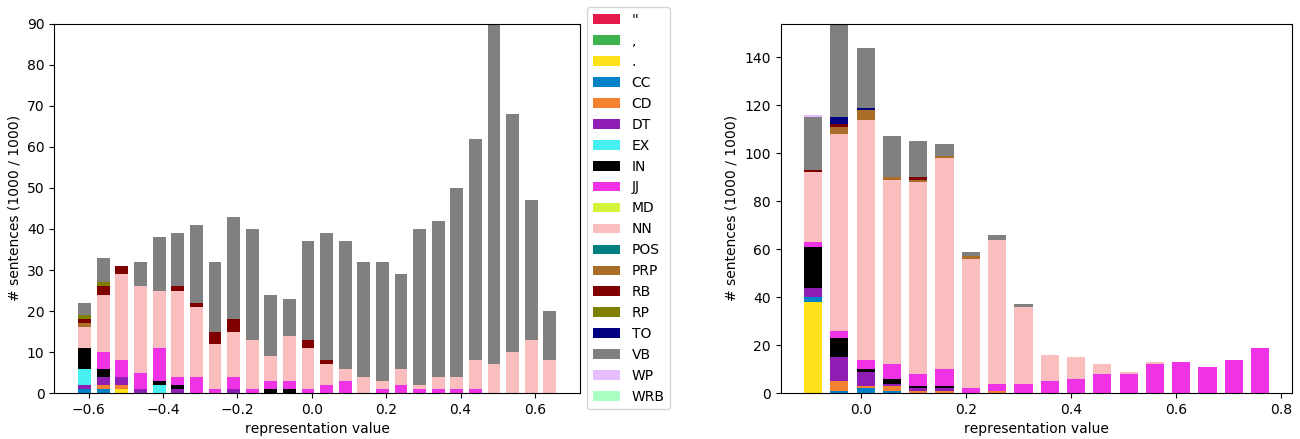
\includegraphics[totalheight=6cm]{fig/find_syntax_vb.png}
	\caption{Dimension 713 encoding verbs (left) and dimension 2020 encoding adjectives.}
	\label{fig:find_syntax_vb}
\end{figure}
Looking at the actual words that are responsible for high values within the dimension however, we find that there is also a semantic commonality between them with verbs mostly being \textit{playing, walking, sitting, running, standing, swimming}. Several interpretations on what they have in common are plausible, like all taaking locations or placies as arguments or all being some kind of physical activity\footnote{Having different scales how physically intensive it is, in the sense of being sportif.}. Nouns scoring high values exclusively denote sprt types like \textit{football, basketball, tennis, baseball, volleyball, hockey}, which represent in combination with a verb also a physical activity. Looking at the words of the adjective-encoding dimension, depicted in Figure \ref{fig:find_syntax_vb} (right) shows an even more obvious semantic relation, since all adjectives\footnote{High valued words of the \textbf{adjective} dimension: young, little, old, small, older, fat, large, elderly, lean, middle-aged, ...} are typically used to describe people, even though many different adjectives do exist in \ac{SNLI}. We face the same problem as described earlier, that different attributes correlate, making a definite interpretation impossible. We also observe that this dimension, as well as others, differs strongly with the gender-specific dimensions in their distributions. Gender-specific dimensions consist of two peaks, intuitively because they encode basically two states, eithher the gender is present or not. This dimension however is encoded using a relatively large range of values, all neing relatively equally represented. Event hough we do not go deeper into a fine-grained analysis of dimensional values, due to the impact arising from encoded contexts, we assume that other information, as in this case, can be scaled. 
\paragraph*{Subjects and objects}
The differentiation between subject and object that can be identified using dependency parsing seems highly useful for classifying image captions. While the subject most likely refers to the main object, depicted in an image, the object may serve as a more informative explanation, however most likely being less relevant. To identify whether the model leanrs equivalent information, we look for subjects and objects respectively. We also look for predicates, however this iss especially noisy since many sentences in \ac{SNLI} actually are noun phrases and thus lack a verb. The closest to encoding this information, even by using dependency parsing labels, was the dimension in Figure \ref{fig:find_syntax_vb}. We find the two dimensions in Figure \ref{fig:find_syntax_subj_obj} for both, subject and object, respectively.
\begin{figure}[tph!]
\centering
	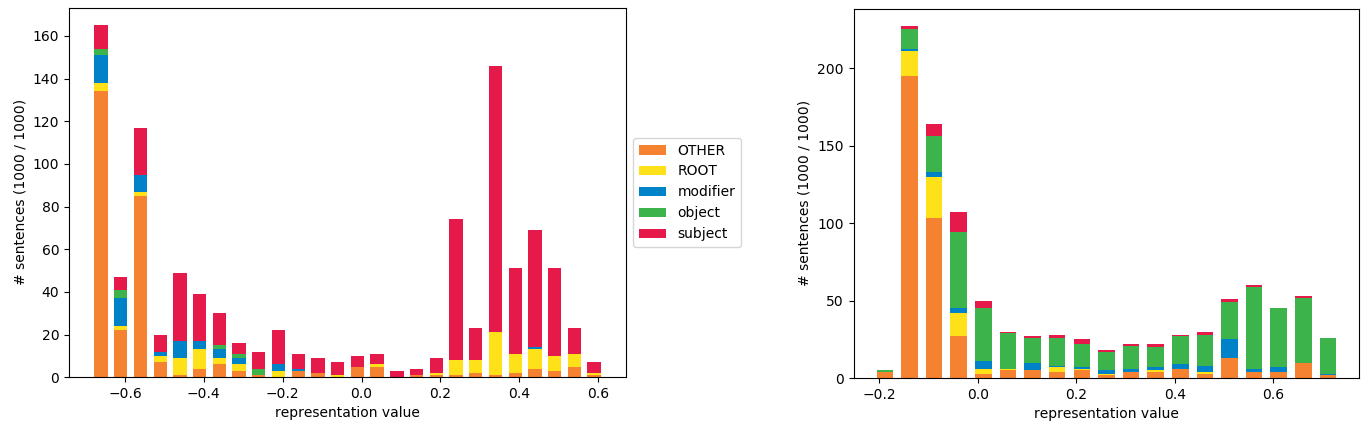
\includegraphics[totalheight=5cm]{fig/find_syntax_subj_obj.png}
	\caption{Dimension 757, encoding the subjects (left), and dimension 1840 encoding objects (right) of sentences.}
	\label{fig:find_syntax_subj_obj}
\end{figure}
Similarily as when analysing the verbal dimension, the first sight suggests that indeed information as from a parse tree is encoded within those dimensions. While this actiually may be true, undeniably both words retrieve high values from words that are also semantically highly related. High dimension of the dimension seemingly encoding ssubjects (left) exlucively contains words referring to people\footnote{High valued words of the \textbf{subject} dimension: man, woman, girl, boy, men, women, boys, girls} when having high values. While they all are very likely to encode a very importnat aspect and subject of the sentence, subjetcs refering to anything else than humans are not considerd by this dimension and it seems more likely that the semantic relationship is encoded and just happens to be the subject. The object-encoding dimension (right) shows the same phenomen, solely encoding words referring to places\footnote{High valued words of the \textbf{object} dimension: street, beach, pool, outside, park, road, restaurant, sidewalk, grass, city, ...} with a high value.
\newline

\noindent
We clearly see that syntactic information is indeed encoded, both for the dependency parse information as well as \ac{POS}. Yet those dimensions highly correlate with semantic and it seems much more likely that the dientification of these semantic patterns is sufficnent for the model to rely on it to encode syntactic information. this obviously is coming from \ac{SNLI} with the majority of sentences regarding people. Another plausible interpretation is that the model does not actually require any syntactical knowledge for the task, based on the simple sentence structure. We conclude that whether the model indirectly uses syntactic information, originating from semantic features, or solely leverages semantic information, not relying on syntax at all, is matter of perspective, the truth lies probably somewhere inbetween. 

\subsection{Insights on the sentence alignment}\label{sec:insights_sent_alignment}
We have shown that dimensions represent a specific information of any kind. High values within these dimensions indicate that the information, encoded by the given dimension, is present while low values indicate it is not present in the sentence. In this section we analyse, using the newly gained insights, how the models finally aligns the encoded information int he sentence represenations to predict the entailment relation label. For our analysis we sample 150 premises, each with one hypothesis for each label respectively, that are all classified correctly by Shortcut-Stacked Encoder\textsuperscript{$\dagger$}. 

\subsubsection{Alignment analysis on a single sample}
We first analyse single samples in order to identify plausible strategies for the network, when mapping both sentence representations, knowing only very little how the network actually leverages from the informtion in the presmise. We demonstrate our results with the samples premise:
\begin{center}
\begin{tabular}{rl}
	\textbf{Premise:} & A woman sitting in the dirt.
\end{tabular}
\end{center}
and its three hypothesis, one for each label:
\begin{center}
\begin{tabular}{rll}
	\textbf{Entailment:} & There is a woman sitting \textit{outside}. \\
	\textbf{Neutral:} & A \textit{dirty} woman sitting in the dirt. \\
	\textbf{Contradiction:} & A woman \textit{standing} in the sand. \\
\end{tabular}
\end{center}
We highlight the words within each hypotheis, that we consider relevant for the label, based on our human judgement. The entailing hypothesis describes for the most part the same setting as the premise. Since \textit{dirt} usually appears \textit{outside}\footnote{Based on its context in conjuntion with ``sitting'', dirt is most likely used in the sense of being a dirty outside ground.}, we consider this change of words as a generalitazion, meaning \textit{outside} includes \textit{dirt} (amongst others). the neutral hypothesis introduces new information about the woman being \textit{dirty}, which is very plausible, yet not explicitely given in the premise. the contradicting hypothesis clearly is cinompatible with the premise, as the woman can either be \textit{standing} or \textit{sitting}, but not both. In this subsection we show that indeed, the identified differences can be easily observed when looking at both sentences simultatneously for the entailing and contradicting hypothesis. For the sake  of brevity we omit the analysis of the neutral sample in this subsection, as it does not give any additional insights.

\paragraph*{Visualizing the entailment relation}
We start by visualizing the relation between the premise and the entailing hypothesis. We assume that the model will rely on the the information encoded within a given dimension to compare the meanings of two sentences and infer its relation. 
\begin{figure}[tph!]
\centering
	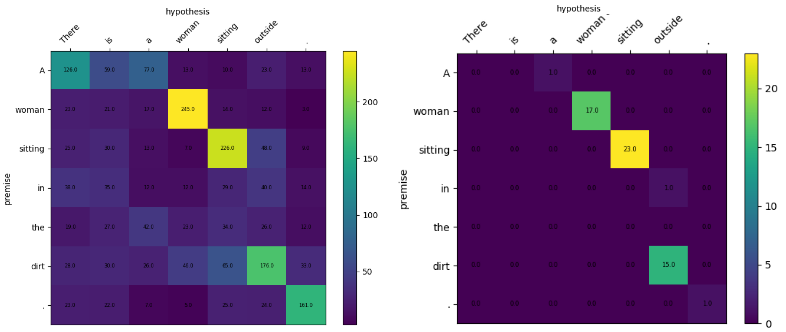
\includegraphics[totalheight=7cm]{fig/alignment_entailment_sample_general.png}
	\caption{Word alignments of an entailing sentence pair either by counting all shared dimensions (left) or only dimensions with at least a value of 0.2 (right).}
	\label{fig:alignment_entailment_sample_general}
\end{figure}
Figure \ref{fig:alignment_entailment_sample_general} (left) shows the alignment between between the premise (y-axis) and the hypothesis (x-axis) by counting all dimensions $d_i$ arising from each word. For eaach word we identify all dimensions $d_i$ that are represented by it in the respresentation. The intersection of a word from the premise and a word of the hypothesis is the total amount of all dimension with the same identifier $i$, that both words represent. thu for instance \textit{dirt} and \textit{outside} have 176 dimensions in common. This plot is quite noisy, since it does not differentiate between different values, thus even dimensions that encode information which is not given in both sentences are arbitrarily aligned between two words. Following our insights from the previous section we filter out all dimensions that do not at least have a value of 0.2 in both sentence representations in Figure \ref{fig:alignment_entailment_sample_general} (right), presumably resulting in only compared information that is present in both sentences. It can be observed that by applying this filtering the main aspects of both sentences (``woman/woman'', ``sitting/sitting'', ``dirt/outside'') are stongly aligned with each other, while the remaining words only show little similarities w.r.t. their encoding. this incidates that aligning both sentences intuitively can result in the entailment label within the examined example.
\newline

\noindent
Note that the actual Shortcut-Stacked Encoder does not only rely on the indial sentence representations but also combines them using element-wise multiplication and difference. 
\begin{figure}[tph!]
\centering
	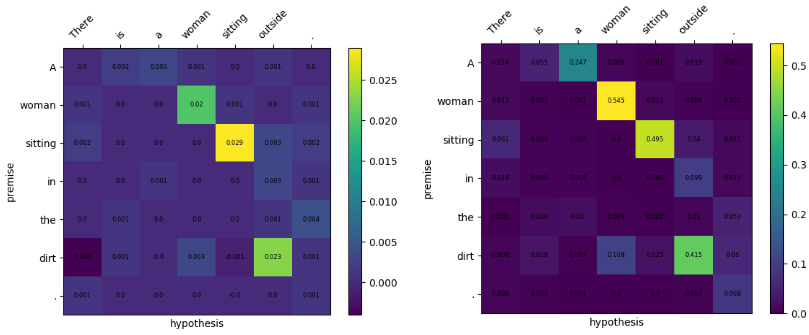
\includegraphics[totalheight=7cm]{fig/alignment_entailment_sample_mult.png}
	\caption{Visualitation of an entailing sample with applied element-wise multiplication either using the mean (left) or maximum (right) product of all shared dimensions for each word pair.}
	\label{fig:alignment_entailment_sample_mult}
\end{figure}
While element-wise difference intuitively serves a direct comparison of the encoded information per dimension, the effect of the multiplication feature is less obvious. Figure \ref{fig:alignment_entailment_sample_mult} (left) visualizes the mean product of both sentence representations using element-wise multiplication as described in Section §\ref{sec:residual_encoder_def}, averaged by the amount of shared dimensions as counted in Figure \ref{fig:alignment_entailment_sample_general} (left). One can observe that the plot arising from element-wise multiplications similarily highlyights the same relevant word relations as seen in the previous plot, indicating that it serves as some kind of soft \texttt{AND}-operator, as it is showing that similar information is present in both sentences. As this plot again might be heavily influenced by irrelevant relations we also visualize the highest elementwise product of all shared dimensions between two words in Figure \ref{fig:alignment_entailment_sample_mult} (right), showing a similar pattern.

\paragraph*{Visualizing the contradicing relation}
We visualize the shared dimensions of both contradicting sentences in Figure \ref{fig:alignment_contr_sample_general} (left) in the same manner as done for the entailment sample, by only counting dimensions that achieve aa value of at least 0.2 for both words of each word-pair. 
\begin{figure}[tph!]
\centering
	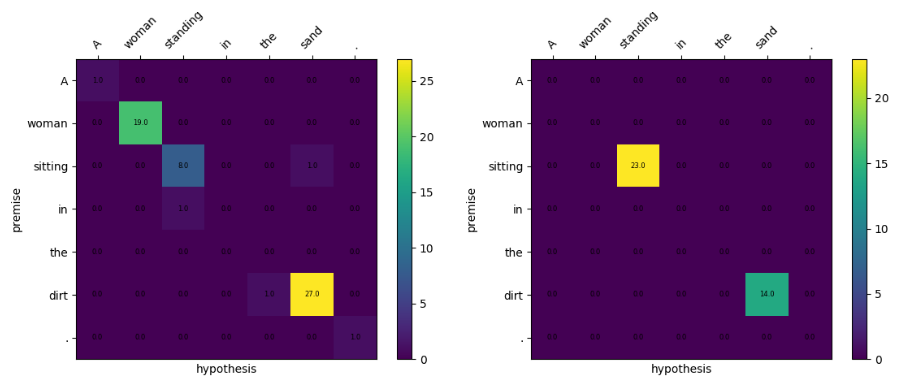
\includegraphics[totalheight=7cm]{fig/alignment_contr_sample_general.png}
	\caption{Visualitation of a contradicting sample by counting meaningful shared dimensions (left) and meaningful distinct dimensions 8right) amongst pairs of words.}
	\label{fig:alignment_contr_sample_general}
\end{figure}
Note that not only the entailing word-pairs show similar values within several dimensions but also \textit{sitting} and \textit{standing} share the same meaning in some cases. This obviously makes sense, as both verbs are similar w.r.t. several aspects. Since the Shortcut-Stacked Encoder creates sentence representations without looking at the other sentence (without inter-sentence attention) it must encode all information that might be relevant and is not able to focus on specific relations that would be crucial for this particular sentence pair. Thus, we also count dimensions that are distinct between two word pairs, depicted in Figure \ref{fig:alignment_contr_sample_general} (right). This is the case for the majority of cases, especially since commpletely unrelated words are encoded by a high amount of distinct dimensions. In order to remove noise coming from this issue we apply two thresholds in our visualization:
\begin{itemize}
\item \textbf{Ensure meaningful relations:} To exclude mthe counts of dimension between unrelated words, we only consider word-pairs with at least 5 meaningful (in the sense of both values reaching at least 0.2) dimensions. This is motivated by the assumtion that the model needs to learn which dimensions can be aligned in a meaningful way, which only is plausible if both words also share at least some commonalities. 
\item \textbf{Ensure meaningful value:} Only considering word-pairs with meaningful relations, we only count dimensions that are distinct for both words if the word of interest reaches at least a value of 0.2, thus encodes information.
\end{itemize}
We observe that indeed \textit{sitting} and \textit{standing} are encoded using  a lot more different than shared dimensions and take a closer look at the actual dimensions in Figure \ref{fig:contradiction_alignment_unshared_dimwise}. 
\begin{figure}[tph!]
\centering
	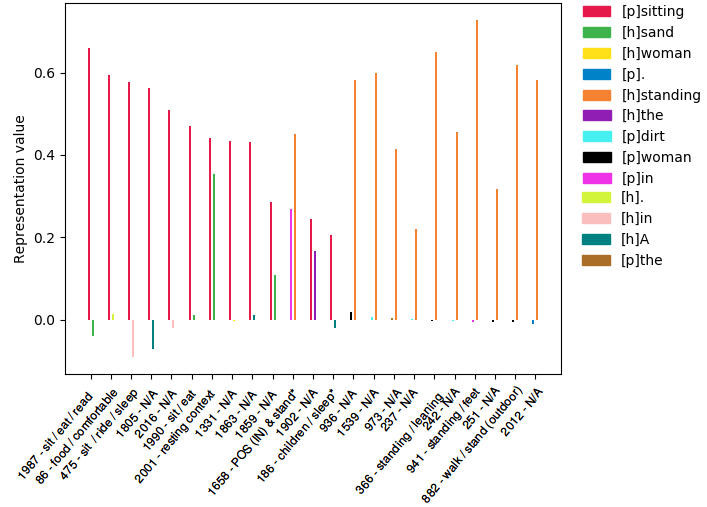
\includegraphics[totalheight=7cm]{fig/contradiction_alignment_unshared_dimwise.png}
	\caption{Dimension-wise visualitation of distinct information represented by \textit{sitting} in the premise and \textit{standing} in the hypothesis.}
	\label{fig:contradiction_alignment_unshared_dimwise}
\end{figure}
The plot shows all dimensions ``meaningful'' dimensions that only encode information coming from one of both words. Each dimensions show two bars, the left bar indicates the value within the representation of $p$, the right bar of $h$. Colors show the word, which is responsible for the value. Additionally we leverage information gained for some dimensions for the previous section, by providing sample words of the general meaning encoded by eaach dimension. We only show these indicators for dimensions that we labelled prior to the visualitation to not be biased towards a specific interpretation. We observe that the identified dimensions indeed highly differ in their value and may be important features to detect contradiction. This plot also is in line with previous conclusions that not-given information results in low values coming from arbitrary words. We also see that the information of what is encoded in the dimensions is helpful for understanding the shown values and do correspond to the responsible word if having a high value.
\subsubsection{Approach for a general alignment understanding}\label{sec:approach_general_alignment_understanding}
Our previous results show that it theoretically is possible for the model  to align relevant dimensions to infer the entailment label and suggest that doing so it can differentite between contradicting or entailing meanings of two sentences. Other than the fact that the model predicted the examined sentence correctly however, our findings are more theoretical than hwo the model actually leverages these information. To also take into account the actual prediction based on the \ac{MLP} we conduct another experiment. Based on our conclusions that high values indicate the presence of a specific information we formulate a very simple form of lexical entailment w.r.t. to our identified encoding schemes. Let $I_p$ and $I_h$ be the sets of information of any kind within $p$ and $h$ respectively. We further assume that lower values within a dimension generally represent less information w.r.t. the information encoded by the dimension:
\begin{enumerate}
\item The hypothesis contains a subset of information ($I_h \subseteq I_p$) would either result in paraphrasing ($I_h \equiv I_p$) or in less specific information in $I_h$, consequently being more general. We expect both cases to be labelled as entailment. We assume that for instance a hyponym \textit{monkey} of the hypernym \textit{animal} contains the same high dimensions as its hypernym and additionally more information that is specific for being a \textit{monkey}.
\item The hypothesis contains a true superset of information ($I_p \subset I_h$) results in the opposite case of the one above. The additional information $I_h \setminus I_p$ is possible true based on the premise, yet not given. We expect this case to be labelled as neutral.
\item The hypothesis and premise contain different information ($I_p \nsubseteq I_h \land I_h \nsubseteq I_p$). We expect the model to predict contradiction if the amount of exclusive information in $I_p$ and $I_h$ is relatively large.
\end{enumerate}

In subsequent sections we will refer to those assumpion using their numbering (1), (2) or (3) respectively. First however, we demonstrate this intuition based on an artifically created sample:
\begin{center}
\begin{tabular}{rl}
\textbf{Premise:} & A \textit{green} man is running on the street.
\\
\textbf{Hypothesis:} & A man is running on the street.
\end{tabular}
\end{center}
This is predicted as entailment, as expected by assumption (1) by our model. After swapping the premise with the hypothesis, the predicted label is neutral, as expected by assumption (2).
\begin{figure}[tph!]
\centering
	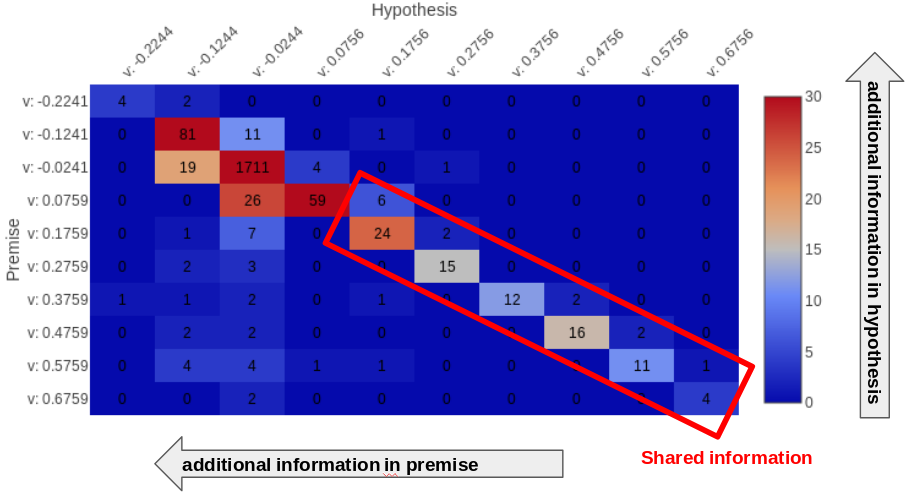
\includegraphics[totalheight=6cm]{fig/sample_coverage_prob.png}
	\caption{Visualitation of a sample sentence pair with explanatory guides for interpretation.}
	\label{fig:sample_coverage_prob}
\end{figure}
We visualize both sentences in Figure \ref{fig:sample_coverage_prob} and include additional hints to explain how this visualtation can be read, as we use will use the same technique when looking at multiple samples simultaneously. intending the figure to serve the validation of our claims, we create it in the following manner: Let $D = \{i \in \mathbb{N} | 1 \leq i \leq n\}$ denote the set of all $n$ dimensions. Furthermore let $p_i$ and $h_i$ denote the value within the $i$th dimension within $p$ and $h$ repsectively. We divide the value range of all values in $\{p_i | i \in D\}$ and $\{h_i | i \in D\}$ respectively into a discrete space using bins of size 0.1, displayed at the y-axis for $p$ and the x-axis for $h$ with their lower bounds. For each $i \in D$ we identify the corresponding bins based on the values $p_i$ and $h_i$ and increment the intersecting field by one. thus, for instance, 1171 dimensions have a value $-0.0241 \leq p_i < 0.0759$ for the premise, while also having a value $-0.0244 \leq h_i < 0.0756$. Following our insights, that low valued dimension encode the absence of information, we consider the uper left corner as irrelevant for the relation classification of both sentences. Arising from the same observations the diagonale, marked by the red recangle, corresponds to information that is present in both, $p$ and $h$. Subsequently, everything that is above this diagonal represents information that only is present within $h$ and accordingly, everything to the left of the diagonale is only present within $p$. We check the origin of all $p_i$ to the left of the diagonal and observe that they exclusively emerge from the word \textit{green}, which is the only additional information, given in $p$.
Knowing that this naive assumption does not completely hold, we evaluate it on the chosen 450 correctly classified examples. While we find evidence for (1) and (2) in some cases, we will show why (3) is not sufficient. 
\subsubsection{Entailment analysis}
We conduct the same experiment as conducted using a single sample in Section §\ref{sec:approach_general_alignment_understanding} over 150 correctly classified mples with the gold label \textit{entailment}. The resulting plot in Figure \ref{fig:entailment_uninversed} is calclualted identically as the plot with thee sample sentences, however displaying the mean amount over all sentence pairs rather than the the absolute amount. We observe that indeed, the majority of sentence pairs contains more information within $p$ than in $h$, undermining our  assumption (1). On the other hand only very few information are present in $h$ and not in $p$. Yet, in order to get a better understanding and seperate entailment relations based on paraphrasing from entailment based on generalitzation we repredict the sentence pairs ($p$, $h$) with premise and hypothesis swapped as ($h$, $p$). 
\begin{figure}[tph!]	\centering
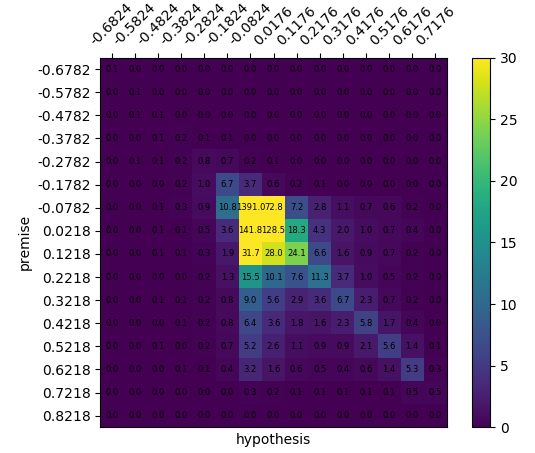
\includegraphics[totalheight=6.5cm]{fig/entailment_uninversed.png}
	\caption{Visualitation of 150 sentence pairs ($p$, $h$), correctly labelled as entailment.}
	\label{fig:entailment_uninversed}
\end{figure}
We expect all sentence pairs that are predicted \textit{entailment} for ($p$, $h$) and ($h$, $p$) to be paraphrasing. We consider all entailing sentence pairs that are \textit{neutral} after swapping to arise from generalitation with the more general sentence $h$ now being the premise. The resulting label distribution after swapping, based on the prediction of the Shortcut-Stacked Encoder\textsuperscript{$\dagger$} is listed below:
\begin{itemize}
\item \textbf{Entailment:} 11 samples (7.3\%)
\item \textbf{Neutral:} 111 samples (74.0\%)
\item \textbf{Contradiction:} 28 samples (17.7\%)
\end{itemize}
Based on the model's prediction th majority of cases are described by the second scenario. Only very few show the same encoding in both sentences. To understand why some samples are predicted as being contradicting after being swapped we take a look at the actual data. As it turns out, in addition to misclassifications, many of the samples contain quite specific $p$ with a highly general $p$, for example (before swapping):
\begin{center}
\begin{tabular}{rl}
\textbf{Premise:} & A girl reaching down into the water while standing at the edge of a river. \\
\textbf{Hypothesis:} & The girl is outside.
\end{tabular}
\end{center}
This should definetly falls into the case of our assumption (2), yet labelling it as contradiction if swapped to ($h$,$p$) may be correct, considering that that while the more specific sentence $p$ entails quite a lot information w.r.t. $h$, making it possible, yet not very likely. Considering that this is a plausible labelling, we conclude the first missing scenario of our assumption, a high amount of extra information in the hypothesis compared to a very broad claim in the premise may be classified as contradiction, rather than our assumption (2) neutral. Looking at the actual data that is now classified as entailment or neutral seems in line with our assumptions (1), (2). Since we are only focusing on these two assumption in this section, we visualize in Figure \ref{fig:alignment_entailment_inversed} samples predicted as entailment (left) and neutral (right) after swapping, since they describe the scenarios we initally intended.
\begin{figure}[tph!]	\centering
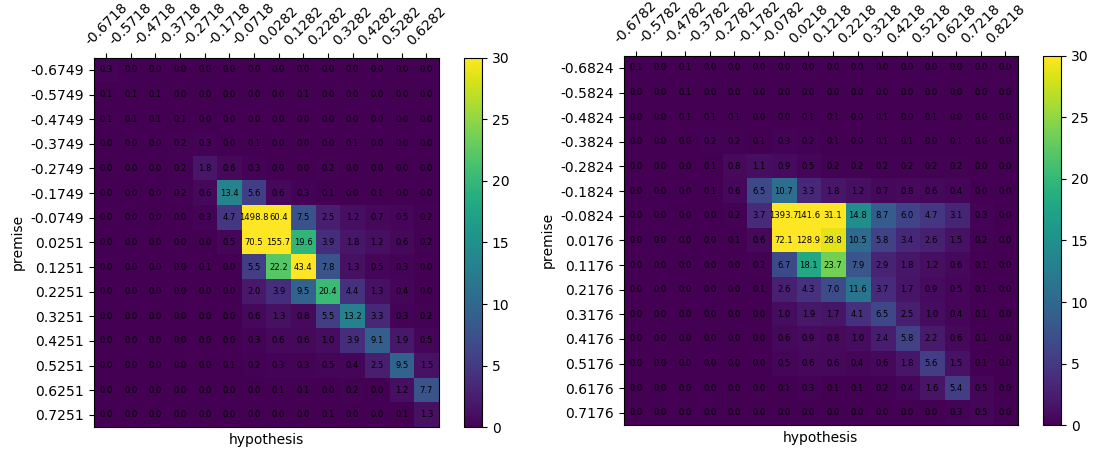
\includegraphics[totalheight=7cm]{fig/alignment_entailment_inversed.png}
	\caption{Visualization of samples predicted as entailment (left) and neutral (right) after swapping $p$ and $h$.}
	\label{fig:alignment_entailment_inversed}
\end{figure}
Indeed, samples that seemingly are paraphrased, based on the model's prediction, show highly identical meaning representations over all dimensions. Similarily, all samples that are now labelled as neutral and before swapping were considered entailment, the vast majority of cases, show a hight tendency of encoding only a subset of information in of the new hypothesis within the new premise. Both plots show that both our assumptions (1) and (2) are correct, accepting the fact that other scenarios exist, as shown by some swapped contradicting samples.
\subsubsection{Neutral and contradiction analysis}
Our previous analysis showed that we can indeed observe how the model identifies the entailing label and to some extend how this differs from neutral and, in one specific setting, from contradiction. We now try to get more insghts on neutral and how it differs from contradiction based on the sentence representations. The results (without swapping) for 150 correctly classified neutral and contradicting examples respectiveely are displayed in Figure \ref{fig:neutr_contr_uninversed}.
\begin{figure}[tph!]	\centering
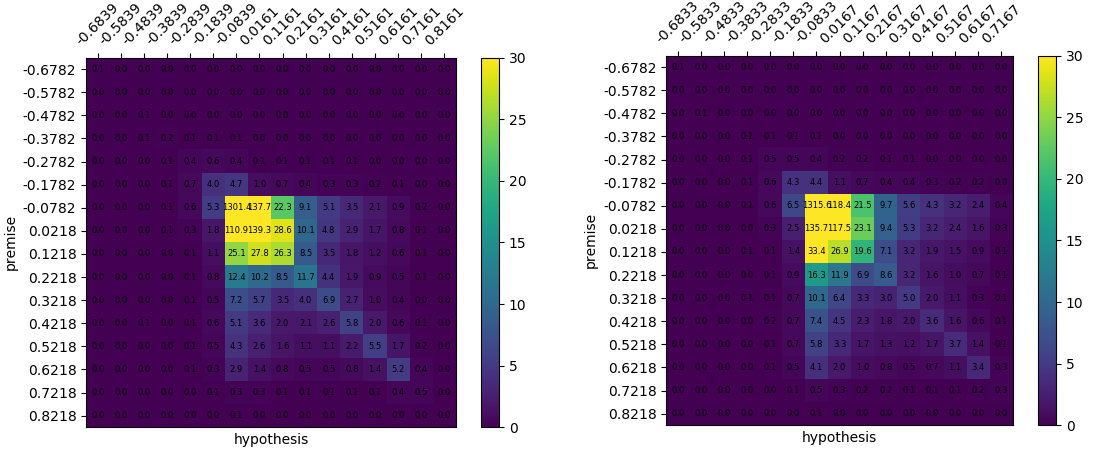
\includegraphics[totalheight=7cm]{fig/neutr_contr_uninversed.png}
	\caption{Visualitazion of 150 sentence pairs ($p$, $h$) correctly labelled as \textit{neutral} (left) and \textit{contradiction} (right).}
	\label{fig:neutr_contr_uninversed}
\end{figure} 
Unfortunately, we do not likewise find any patterns and also do not succeed by seperating them for a more detailed analysis into smaller subgroups. This does not mean that our assumption (3) is incorrect, since indeed contradicting samples show very distinct information in $p$ and $h$. Yet the same thing obviously happens for the neutral label. It  might be slightly less distinct information when looing at the absolute numbers, however this difference is far from being representative. We find an explanation for this issue by looking into the samples. Consider the following two samples, classified correctly as neutral:
\begin{center}
\begin{tabular}{lr}
\textbf{Premise} & A group of kite surfers are busy surfing some waves. \\
\textbf{Hypothesis} & The kite surfers are participating in a race. \\
\midrule
\textbf{Premise} & A baby laughing on the floor. \\
\textbf{Hypothesis} & A baby is being tickled.
\end{tabular}
\end{center}
In both cases, premise and hypothesis do contain distinct information, yet this information is not mutually exclusive but highly compatible with each other and in fact may also be true. We also look at correctly classified contradicting samples:
\begin{center}
\begin{tabular}{lr}
\textbf{Premise} & A boy eating at a table. \\
\textbf{Hypothesis} & A boy coloring at a table. \\
\midrule
\textbf{Premise} & A baby laughing on the floor. \\
\textbf{Hypothesis} & A toddler is crying.
\end{tabular}
\end{center}
Also in this case both sentences encode different information, this time however it is not compatible, as the baby is either \textit{laughing} or \textit{crying} and the boy is either \textit{eating} or \textit{coloring}, but not both things. We see that assumption (3) holds for contradiction in terms of recall, however it is not sufficient to distinguish between neutral and entailment. We conclude that in order to do so, it has to be identified which dimensions can be true simultaneously, indicating neutral, and which dimensions exclude each other, indicating contradiction. in order to see how this is done within the model we need to understand the \ac{MLP} on top of the sentence representation. This however goes back to the main drawback of standard neural networks being hard to interpret and we end our model understanding analysis at this point.
%\subsubsection{Experiments}
\subsubsection{Summarizing the inisghts onmMax-pooled sentence representations}
We have shown that it is possible to identify the general meaning of a dimension based on the words of a sentence, responsible for the dimensions value. We observe that high vlues within dimensions encode the presence of information, which intuitively goes with the nature of the max-pooling mechanism, while low values indicate the absence of information. In an experiment we additionally have shown that knowing the encoding-scheme and information of a dimension, it is possible to change sentence representations in meaningful intended way, yet observed minor side-effects. in the second section we showed that by aligning dimensions and knowing their encoded information, it is possible to understand sentence represeentations well enough to interpret the prediction reason. In the last part we analysed how the model actually performs the alignment between the sentence representation and showed intuitive explanations for some cases of relatedness between both sentences.
\newline

\noindent
All these results are based on a rather small amount of rather small sentences, stemming from \ac{SNLI} and thus merely show experimental results. For a general claim similar experiments should be conducted on larger size and range of data, especially containing longer text, using different models (all with max-pooled sentence representation) to see if those claims still holds. 
\subsection{Identification of missing knowledge}
In order to see what information is not captured by the model and can be helpful for integration we analyse the errors made on \ac{SNLI}. This analyses uses Shortcut-Stacked Encoder\textsuperscript{$\dagger\dagger$}, being closer to the reported accuracy by \cite{nie2017shortcut}. 
\subsubsection{Approach}
Aiming for missing knowledge and not for a general error analysis we focus on misclassified samples with gold label contradiction, predicted as entailment and vice versa, as we find that the label neutral was overall not that well understood by the \ac{SNLI} annotators. To simplify the process we sample according to this constraint sentence-pairs having a high lexical overlap\footnote{Only considering a sentence pair if at least 50\% of the words within the shorter sentence are contained in the other sentence in a \ac{BoW} perspective. Casing is ignored.} and look for the knowledge required by a human to predict the correct label. In total we look at 196 samples incorrectly predicted as entailment and 163 samples incorrectly predicted as entailment identify common categories of missing knowledge. Note that by prefiltering the samples this way, our results exclude certain aspects. For instance many contradicting samples have multiple exclusive elements, resulting in a low lexical overlap.
\subsubsection{Quantitative results}
We show our quantitative results with the identified categories incuding sample sentence pairs for both labels in this section.

\paragraph*{Misclassified contradicting samples}
Table \ref{tab:misclassified_orig_contr} shows the misclassifications of samples labelled incorrectly as entailment.
\begin{table}[tph!]\label{tab:misclassified_orig_contr}
\centering
\begin{tabular}{cccl}
\textbf{Problem} & \textbf{Type} & \textbf{Amount} & \textbf{Example} \\
\toprule
cohyponym & Nouns & 29 & \specialcell{A \textit{creek} runs through the grassy area.\\A \textit{lake} appears in the grassy area.}\\
cohyponym & Verbs & 32 & \specialcell{The boy is \textit{riding} his skateboard.\\The boy is \textit{carrying} his skateboard with him.}\\
cohyponym & Amounts & 33 & \specialcell{\textit{Three} people resting on a snowy mountain.\\\textit{Four} people are on a snowy mountain.}\\
antonym & Adjectives & 13 & \specialcell{The ground is \textit{covered} in snow.\\The ground is \textit{visible}.}\\
antonym & Verbs & 14 & \specialcell{boy \textit{pushing} wagon with two pumpkins in it\\A boy is \textit{pulling} a wagon with two pumpkins in it.}\\
antonym & Prepositions & 17 & \specialcell{A man walking \textit{down} stairs.\\The man is walking \textit{up} the stairs.}\\
\midrule
structure & All & 15 & \specialcell{a sheep chases a dog.\\There is a dog chasing a sheep.}\\
common sense & All & 20 & \specialcell{Someone in a 3ft swimming pool.\\A person is in a very large and deep pool.}\\
\midrule
\textit{ignored} & \textit{ignored} & 23 & \specialcell{A man climbing a rock wall.\\A man climbs the wall.}\\
\midrule
\textbf{Total} & - & \textbf{196} & - \\
\bottomrule      
\end{tabular}
\caption{Misclassified samples with gold label \textit{contradiction}, predicted as \textit{entailment}.}
\end{table}
We find that most problems arise from words sharing lexical relations, namely antonomy or cohyponomy for different kind of \ac{POS}. We opt to show \textit{Amounts} as a seperate category, due to its high frequence. While Verb antonyms may also be considered as cohyponyms, we also list them seperately, if they refer to the opposite meaning. Some samples, listed under \textit{structure} require the model to take word order into consideration, and is mostly represented by semantic role reversal. We assign all samples to \textit{common sense}, that requires information that cannot be retrieved using lexical semantic relations and usually need additional information, implied by the described entity or activity. Any sentence pair were we could not identify the required knowledge, due to not agreeing with the label, highly ungrammatical  sentences or some rare very specific details are ignored in our results, categorized as \textit{ignored}.

\paragraph*{Misclassified entailing samples}
Analysing the required knowledge for misclassified entailing samples as contradtiong, we identify different categories, depicted in Table \ref{tab:misclassified_orig_ent}.
\begin{table}[tph!]
\centering
\label{tab:misclassified_orig_ent}
\begin{tabular}{cccl}
\textbf{Problem} & \textbf{Required knowledge} & \textbf{Amount} & \textbf{Example} \\
\toprule
Paraphrasing & lexical knowledge & 16 & \specialcell{Two people play \textit{foosball}.\\Two people are playing \textit{table soccer}.}\\
\specialcellc{Paraphrasing\\(negated opposite)} & lexical knowledge & 19 & \specialcell{A young boy is \textit{sleeping}.\\A child is \textit{not awake}.}\\
Paraphrasing & world knowledge & 20 & \specialcell{girl \textit{opening} cosmetics \textit{bottle}\\The girl is \textit{removing the top} off the \textit{bottle}.}\\
Generalization & lexical knowledge & 30 & \specialcell{The two \textit{boxers} are females.\\There are two female \textit{athletes}.}\\
Implication & world knowledge & 53 & \specialcell{A hockey player makes a shot.\\A hockey player \textit{is on ice}.}\\
\midrule
\textit{ignored} & \textit{ignored} & 25 & \specialcell{two people sit on a bench.\\two people sit on sand near water.} \\
\midrule
\textbf{Total} & - & \textbf{163} & - \\
\bottomrule      
\end{tabular}
\caption{Misclassified samples with gold label \textit{entailment}, predicted as \textit{contradiction}.}
\end{table}
Essentially we find three different ways, of how the relation between $p$ and $h$ can be described and we differentiate between lexical- and world-knowldge being required for the correct prediction. In the example of paraphrasing, for \textit{foosball} and \textit{table soccer} or \textit{sleeping} and \textit{awake} it is sufficient to detect that they are synonyms or antonyms respectively. The third case required some actual understanding of the process of \textit{opening} in the context with a \textit{bottle}. While some of these samples may be understood by lknowing several meronyms, we consider them to require a deeper conceptual understanding of how thing work. The largest group also is interesting, as all $h$ contain additional information, not directly given by $p$. While this case should usually be labelled as neutral, in this case the additional information is automatically implied\footnote{For the given sample, we assume that Americans see \textit{hockey} in the sense of \textit{ice-hockey}.} (even though not textual) by $p$. This implication also required other external knowledge than lexical relations.

\subsubsection{Conclusions}
We observe that especially the classification of contradicting samples can be improved by using lexical relations, which are available in WordNet, as described in Section §\ref{sec:wordnet}. While those may partially be helpful for the entailing samples, in their case world-knowledge seems more relevant, as could be gained from resources like Wikipedia (see Section §\ref{sec:wikipedia}). While obviously the goal of \ac{NLI} is, to have proper reasonng capabilities, capable of dealing with world knowledge, we emphasize the aspect of lexical knowledge, arguing that any insights on how to incporporate this (simpler) information may later be applied used to include world-knowledge.
\newline

\noindent
Note that the identified problems with lexical relations, especially \textit{antonomy} and \textit{cohyponomy} in Table \ref{tab:misclassified_orig_contr}, refer to the same problem, stemming from the nature of distributed representations. Essentially, they follow the distributional hypothesis, described by \cite{pantel2005inducing} as 
\begin{quotation}
\textit{``[...] words that occur in the same contexts tend to have similar meaning.''}\citep{pantel2005inducing}
\end{quotation}
Considering a sentence like ``The president of Italy hopes to get re-elected.'', one can easily conclude that \textit{Italy} is a country based on its context. Even replacing \textit{Italy} by any made-up country would intuitively result in the same conclusion. Subsequently to being represented by their context words, distributed embeddings supposedly have better generalization abilities \citep{lecun2015deep} due to encoding this phenomen. However also mutually exclusive co-hyponyms or antonyms often share similar contexts (like most countries could replace \textit{Italy} in the given example), resulting in very similar vector representation despite opposite meanings. This is a known problem \citep{sahlgren2008distributional} of distributed word representations and several approaches, as explained in Section \ref{sec:embeddings_improvements_relwork}, aim to fix these problems in the embedding space.